\documentclass[landscape]{foils} 
\input{../common-preamble-start}
\input{../preamble.tex}
\usepackage{url}
\usepackage{hyperref}
\hypersetup{backref,  linkcolor=blue, citecolor=red, colorlinks=true, hyperindex=true}

\begin{document}
\pagecolor{white}
\unitlength=1mm
\begin{center}
{\Large Many of the  slides that I'll use have been borrowed from Dr.\ Paul Lewis, Dr.\ Joe Felsenstein. Thanks!}
\vskip 15mm
\large Paul has many great tools for teaching phylogenetics at his web site: \\
\url{http://hydrodictyon.eeb.uconn.edu/people/plewis}
\end{center}

\myNewSlide

\section*{Do desert green algae use xanthophyll to protect against excessive light intensities?}
\begin{center}
\begin{tabular}{|c|c|c|}
	\hline
	Species \hskip 2mm & Habitat \hskip 4mm & Photoprotection\\
	\hline 1 & terrestrial & xanthophyll \\
	\hline 2 & terrestrial & xanthophyll \\
	\hline 3 & terrestrial & xanthophyll \\
	\hline 4 & terrestrial & xanthophyll \\
	\hline 5 & terrestrial & xanthophyll \\
	\hline 6 & aquatic & none \\
	\hline  7 & aquatic & none \\
	\hline 8 & aquatic & none \\
	\hline  9 & aquatic & none \\
	\hline 10 & aquatic & none \\
	\hline
\end{tabular}
\end{center}

\myNewSlide
\section*{Phylogeny reveals the events that generate the pattern}
\begin{picture}(0,0)(0,0)  \put(-15,-65){\makebox(0,0)[l]{\includegraphics[scale=1.2]{../nonfreeimages/pol/char_correlation.pdf}}}
\put(-25,-140){1 pair of changes.}
\put(-25,-150){Coincidence?}
\put(110,-140){5 pairs of changes.}
\put(110,-150){Much more convincing}
\end{picture}

\myNewSlide
\section*{Inferring Process from Pattern}
{\large
Hypothesis:\par
	Gregariousness should arise more frequently in unpalatable organisms than in tasty ones \citep{SillenT1988}
}

\myNewSlide
\section*{Inferring Process from Pattern}
\begin{picture}(-0,0)(-0,0)
	\put(0,0){\makebox(30,-150)[l]{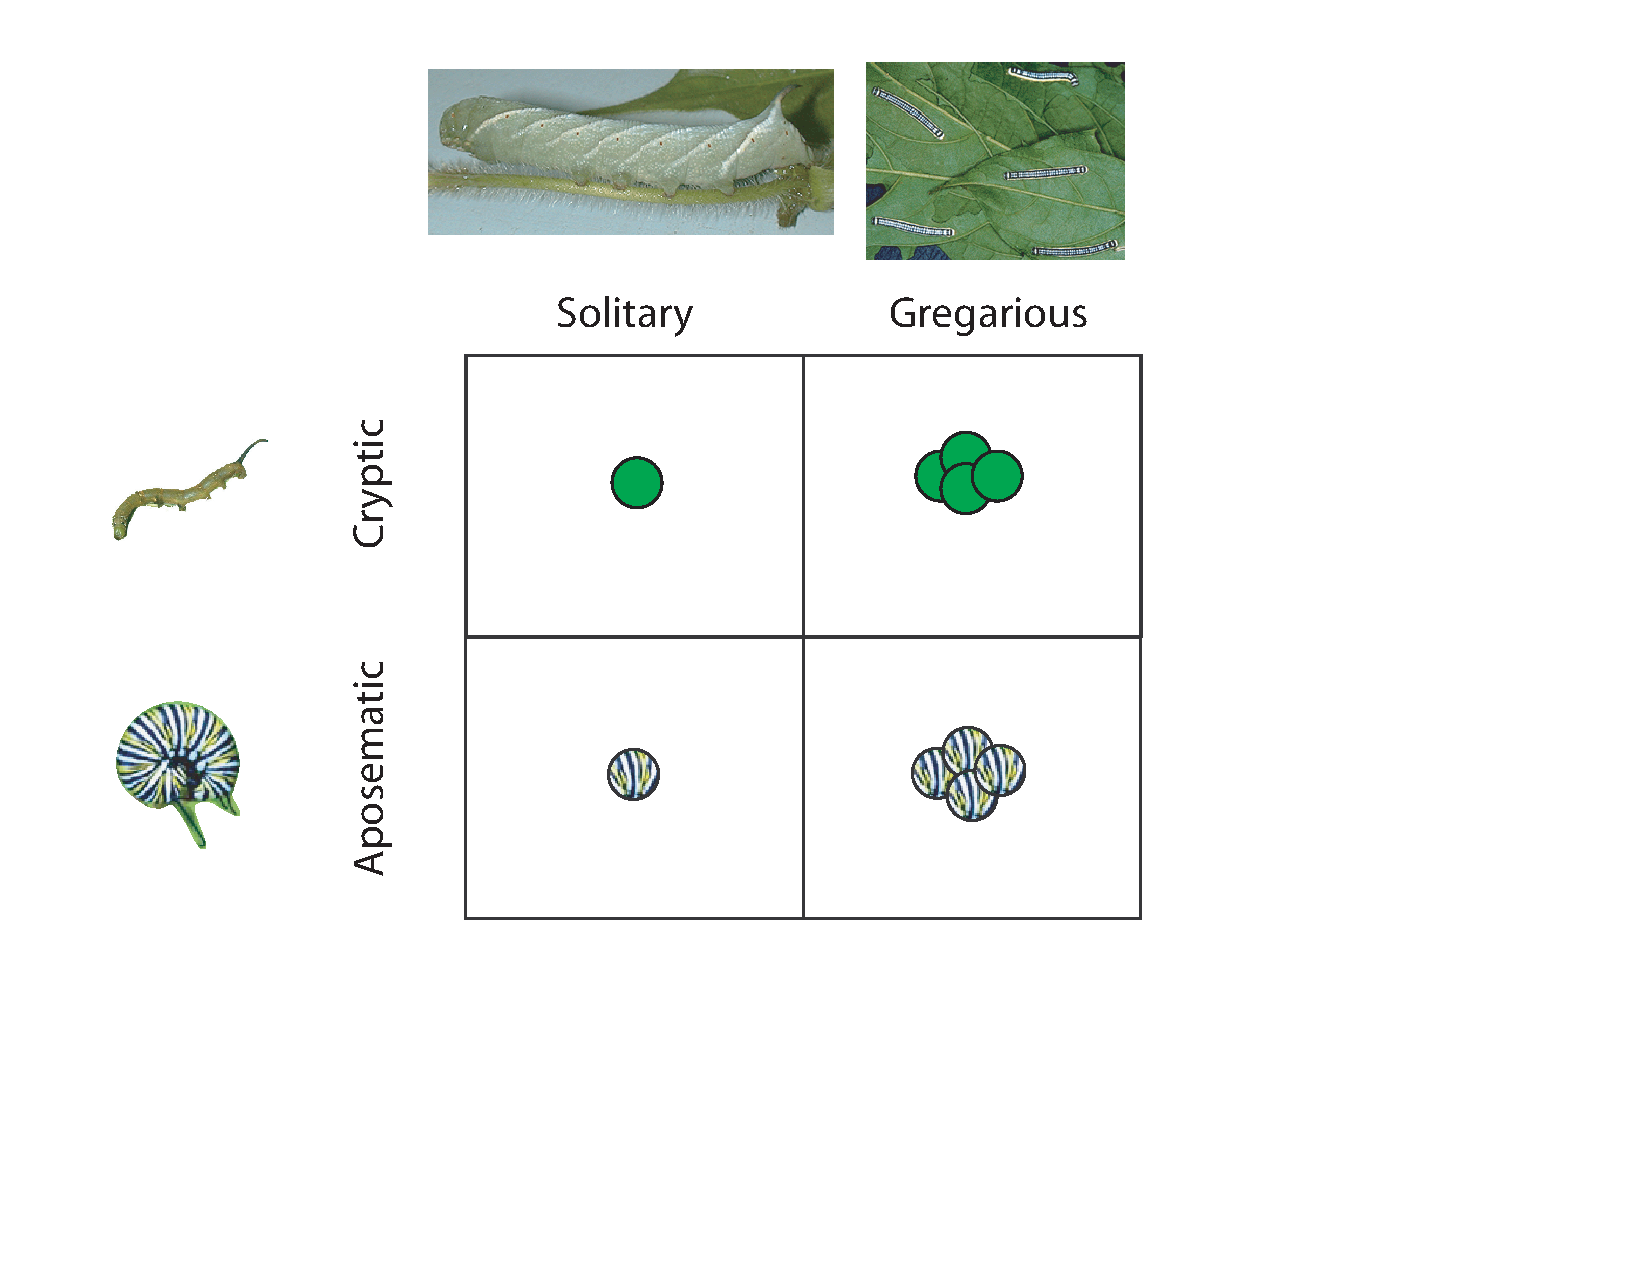
\includegraphics[scale=1.]{../images/cat_legend.pdf}}}
	\put(25,-145){\small \citet{SillenT1988}, \citet{Dyer2002}, \citet{Hill2001}}
\end{picture}


\myNewSlide
\section*{Inferring Process from Pattern}
Some (fake) data:\\
\begin{picture}(-0,0)(-0,0)
	\put(-50,-150){\makebox(10,-150)[l]{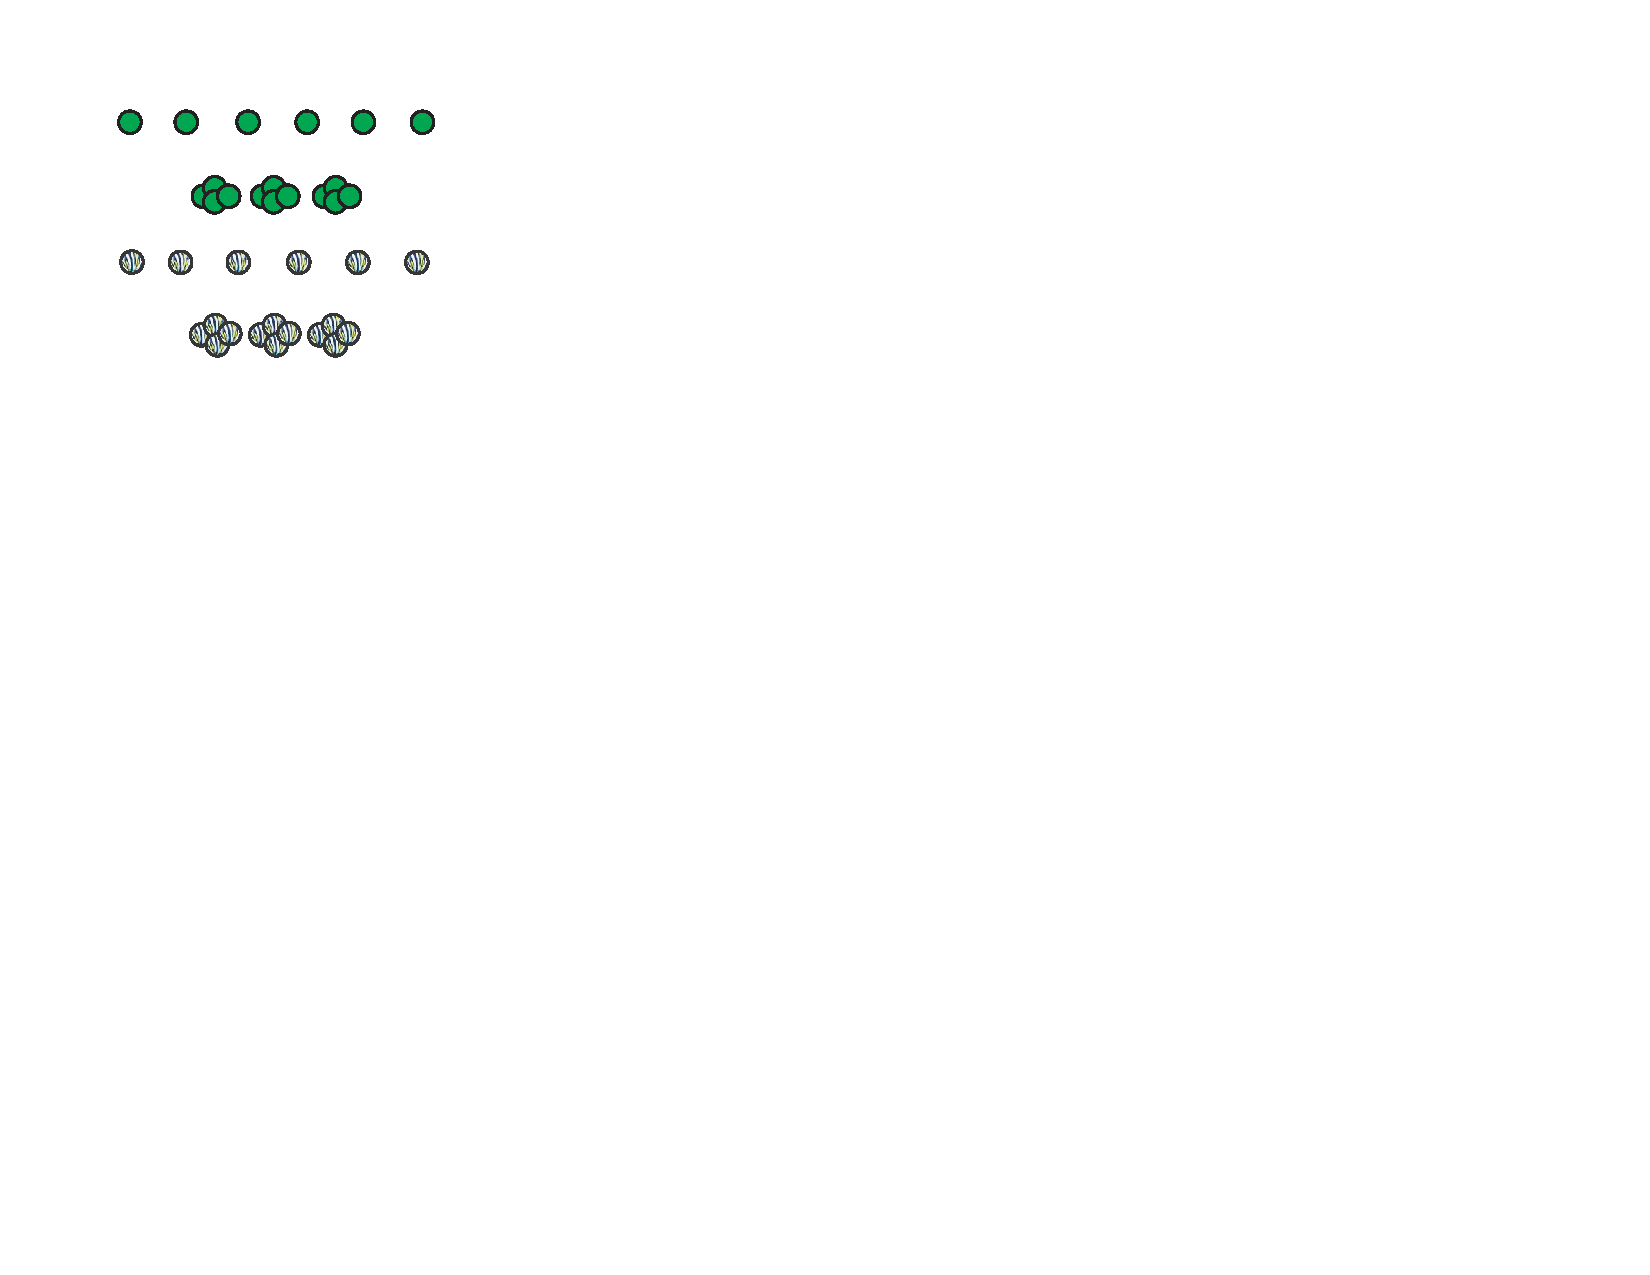
\includegraphics[scale=2.4]{../images/nonPhylogeneticData.pdf}}}
	\put(130,-18){6 cryptic, solitary species}
	\put(130,-47){3 cryptic, gregarious species}
	\put(130,-75){6 aposematic, solitary species}
	\put(130,-105){3 aposematic, gregarious species}
\end{picture}

\myNewSlide
\begin{picture}(-0,0)(-0,0)
	\put(-10,-60){\makebox(30,-150)[l]{\includegraphics[scale=1.4]{../images/noassoc.pdf}}}
	\put(5,-170){One possible outcome:  }
	\put(10,-180){No clear evidence of associations between traits}
\end{picture}

\myNewSlide
\begin{picture}(-0,0)(-0,0)
	\put(-10,-60){\makebox(30,-150)[l]{\includegraphics[scale=1.4]{../images/stTree.pdf}}}
	\put(5,-170){Cartoon of the real results \citep{SillenT1988}}
	\put(5,-180){Aposematic species are more likely to evolve gregarious larvae}
\end{picture}

\myNewSlide
\section*{Importance of phylogeny}
The previous slides had identical patterns of traits if the phylogeny is ignored.

Without knowledge of the tree, no conclusion would be reached.

\myNewSlide
\bibliography{../phylo848}

\end{document}


\myNewSlide
\begin{picture}(0,0)(0,0)
	\put(-50,-185){\makebox(0,0)[l]{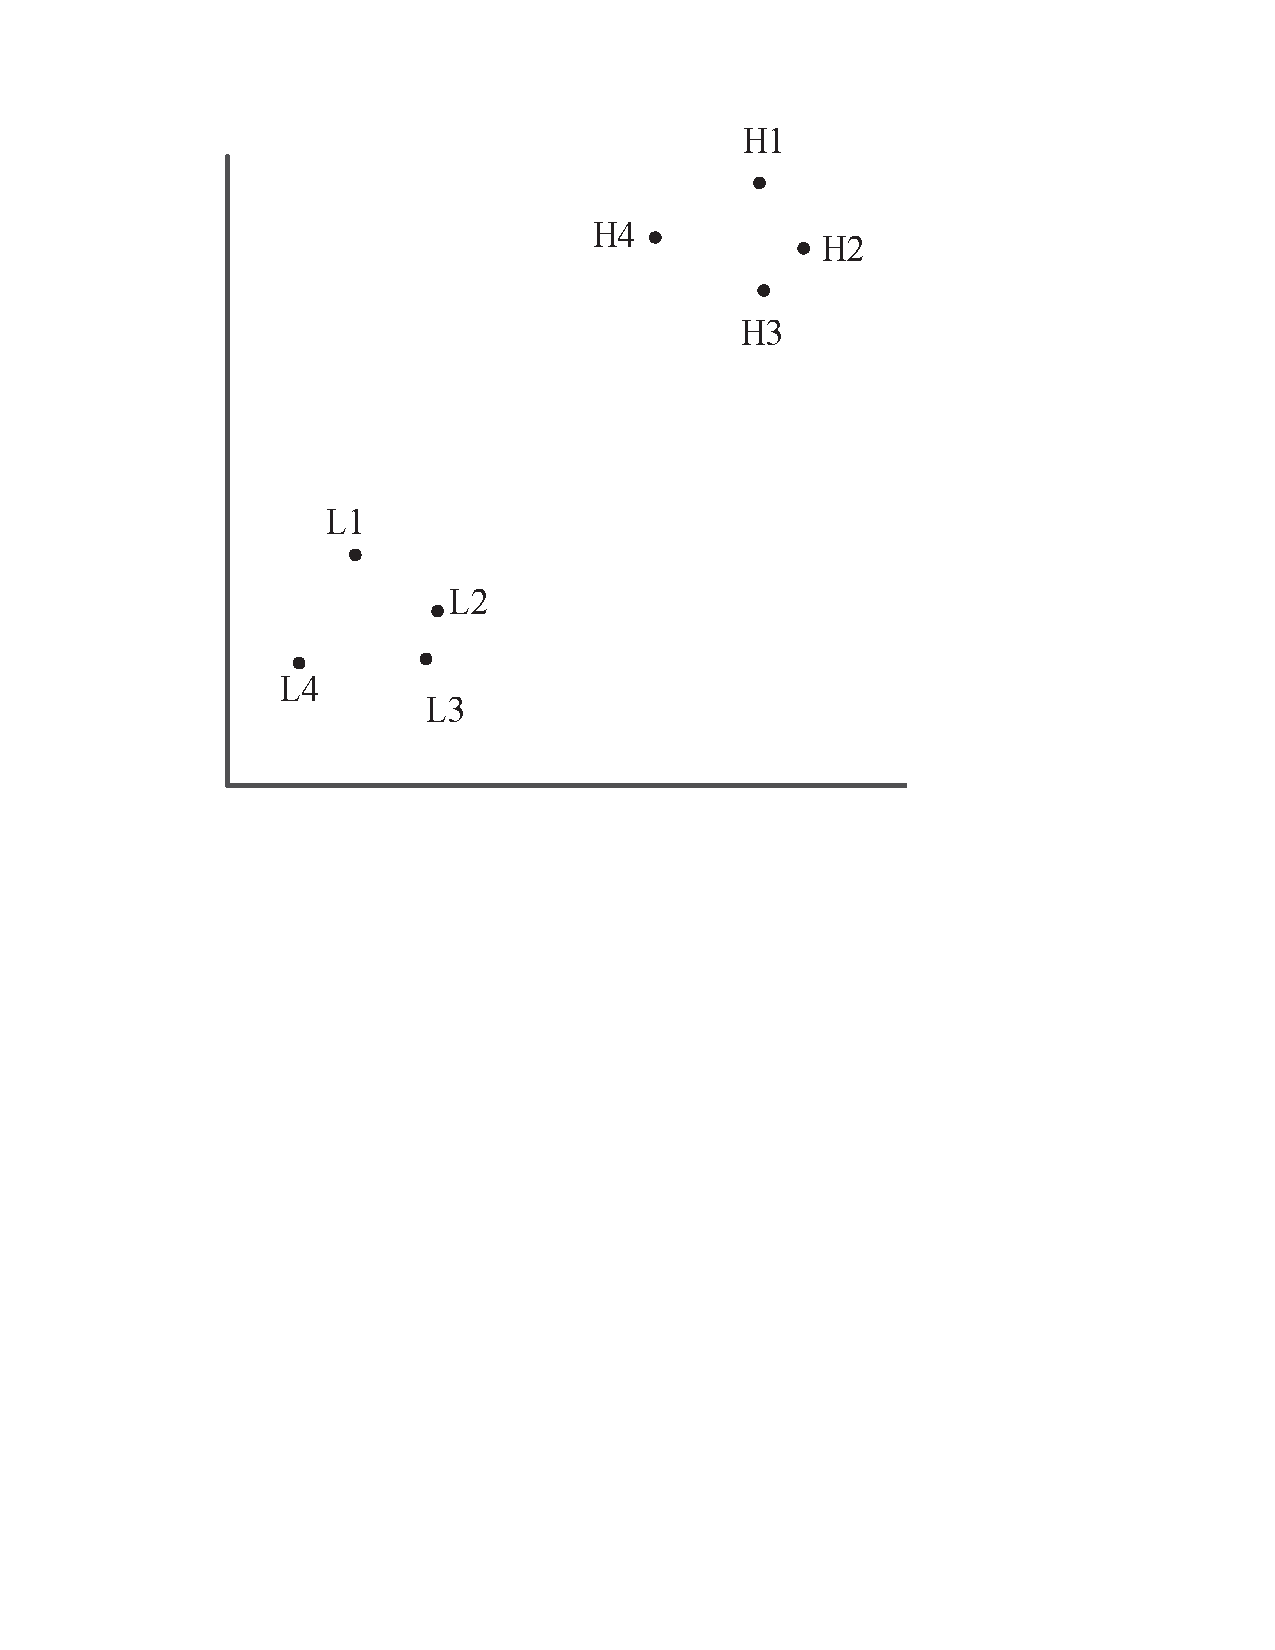
\includegraphics[scale=1.5]{../images/pattern.pdf}}}
\end{picture}

\myNewSlide
(cue cartoon videos)
\myNewSlide
\section*{No (or little) evidence for correlation}
\begin{picture}(0,0)(0,0)
	\put(-20,-145){\makebox(0,0)[l]{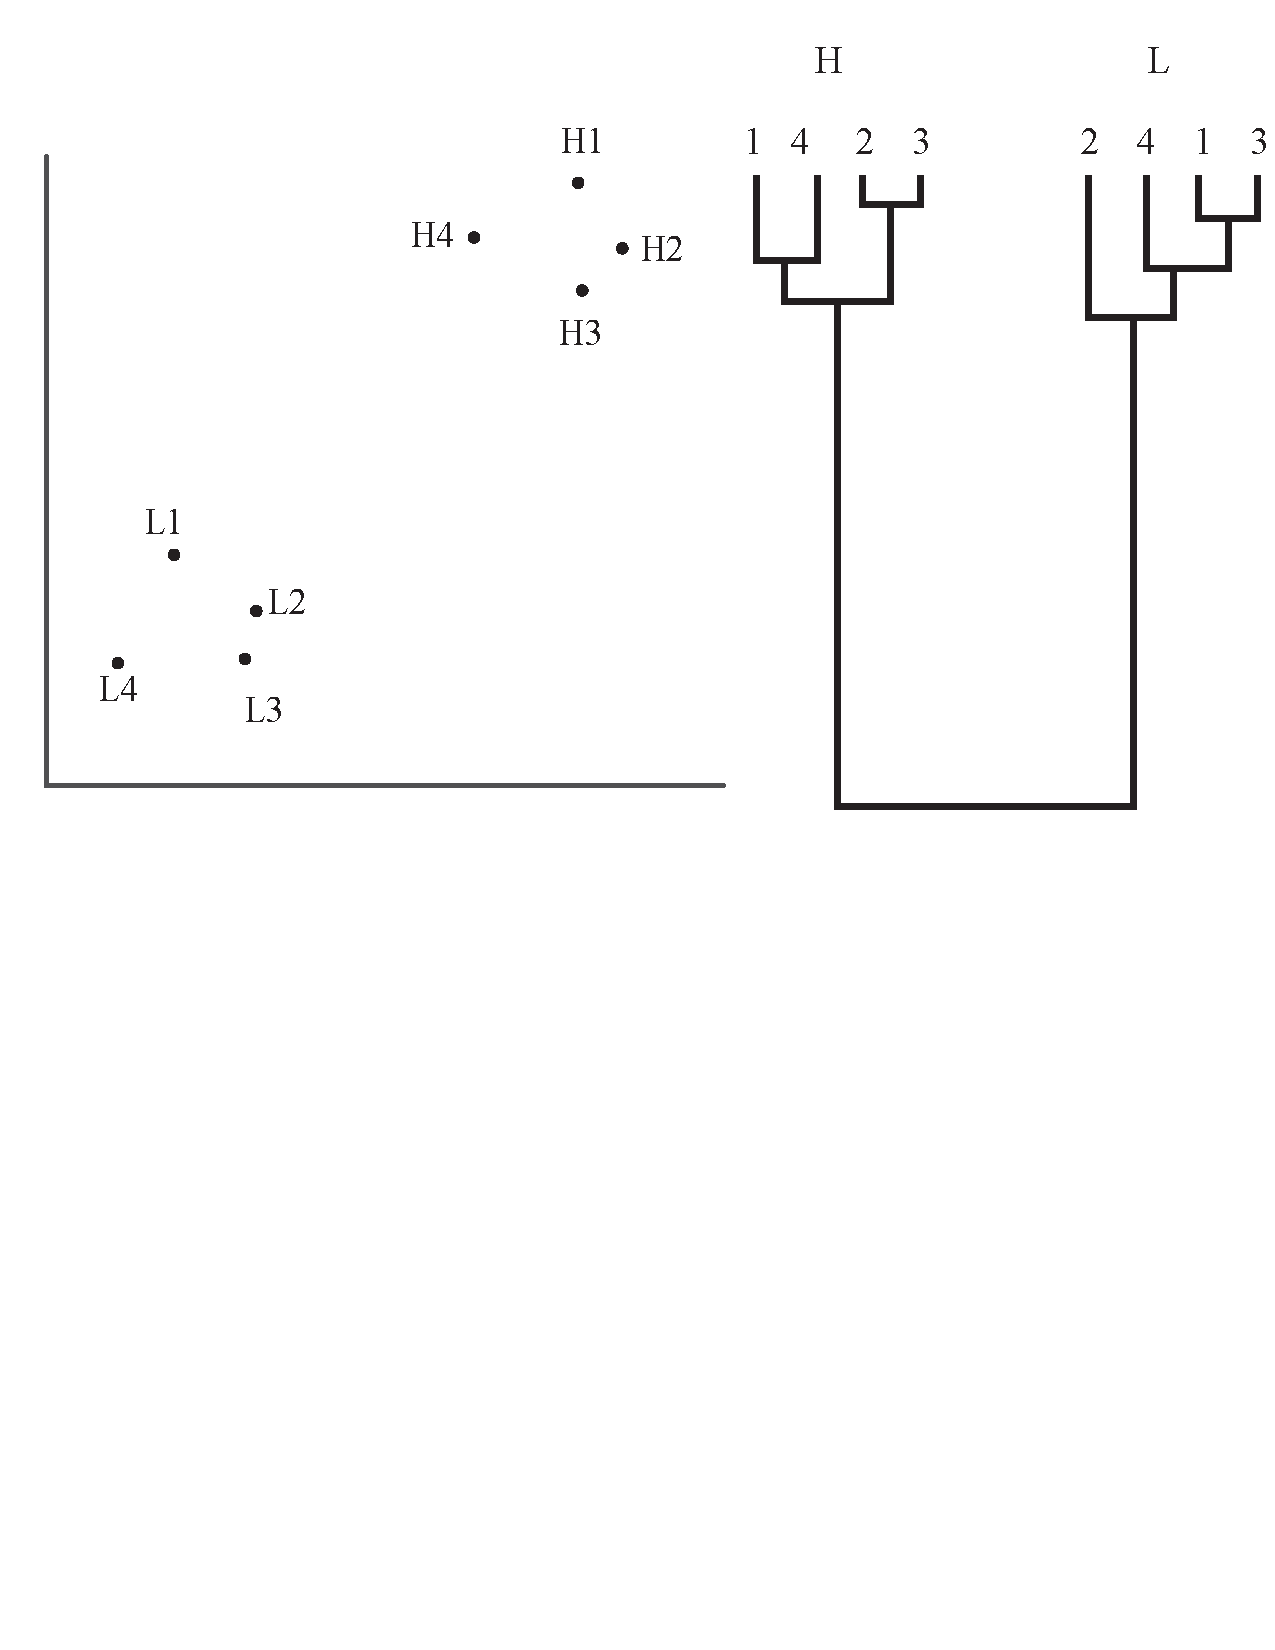
\includegraphics[scale=1.2]{../images/pattern-no-correl.pdf}}}
\end{picture}

\myNewSlide
\section*{Evidence for correlation}
\begin{picture}(0,0)(0,0)
	\put(-20,-145){\makebox(0,0)[l]{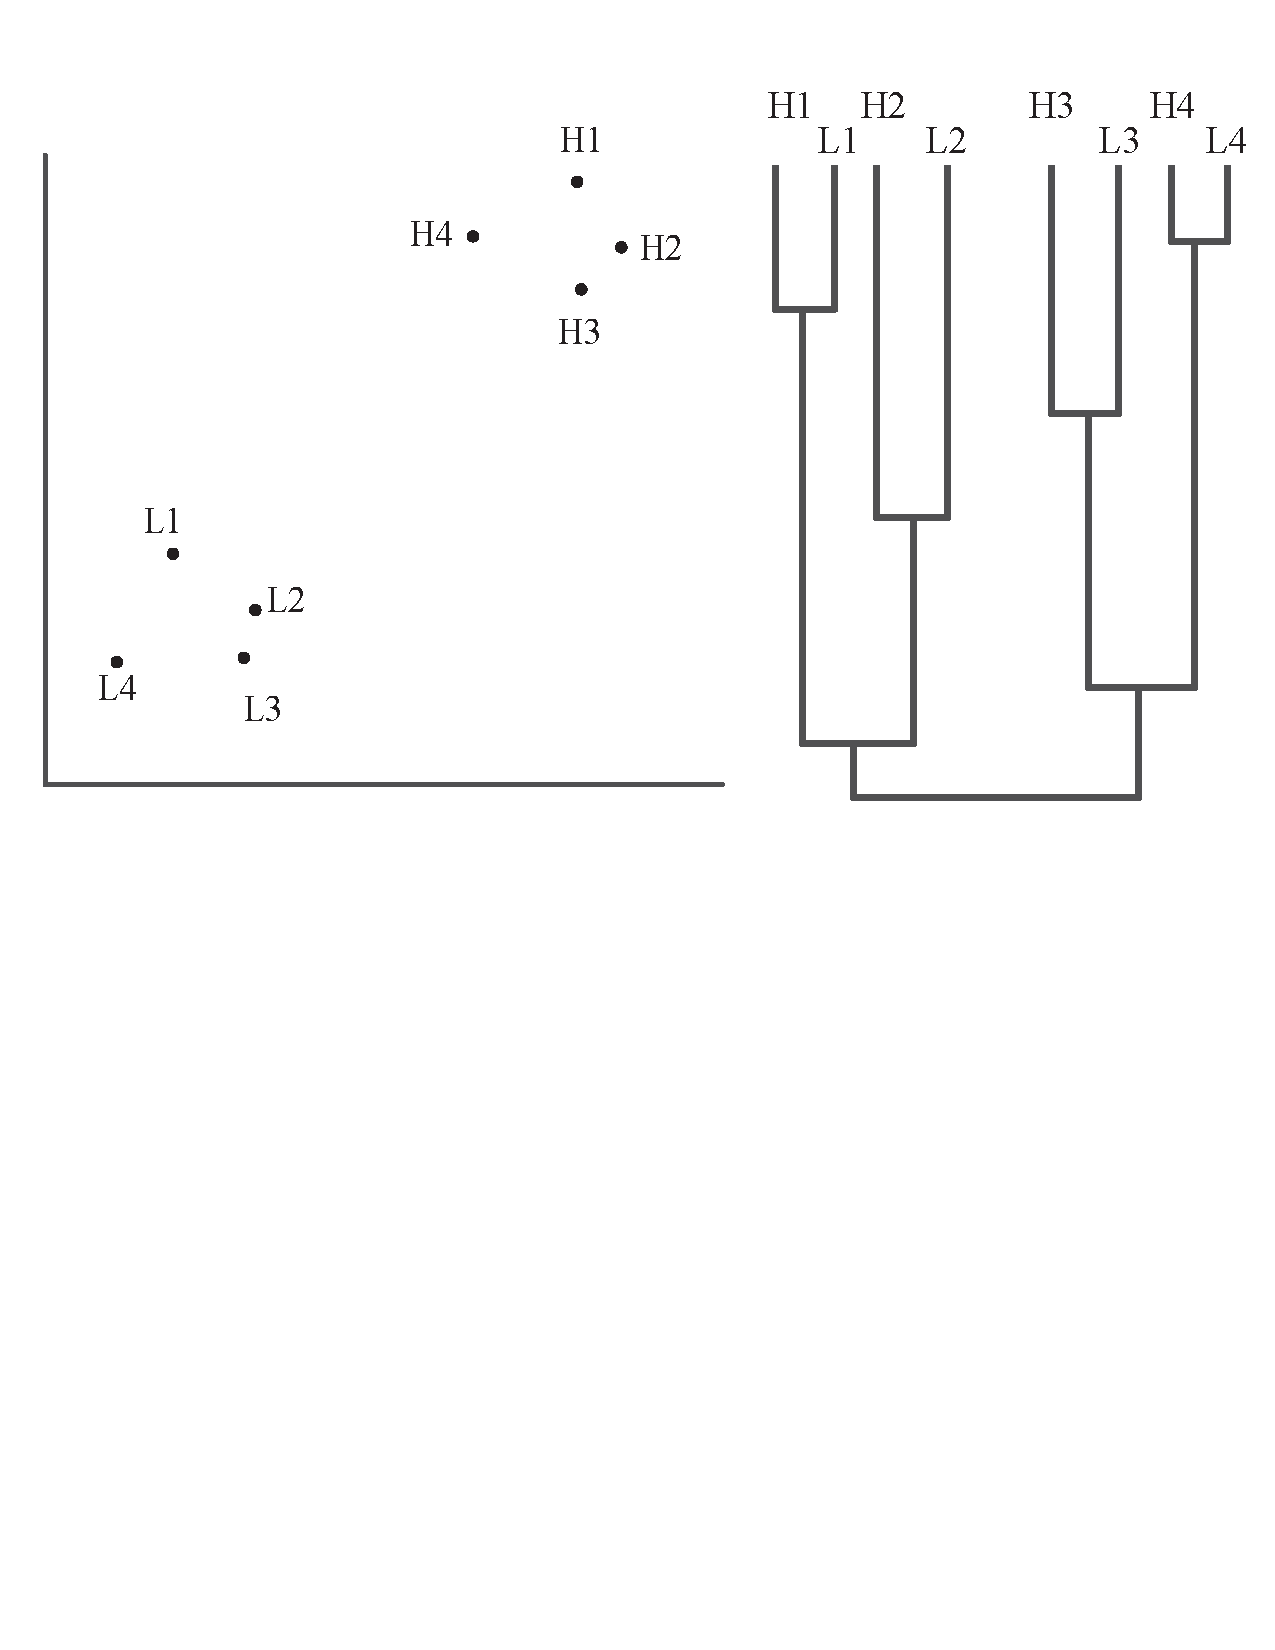
\includegraphics[scale=1.2]{../images/pattern-correl.pdf}}}
\end{picture}


\myNewSlide

\begin{picture}(0,0)(0,0)
	\put(-5,-85){\makebox(0,0)[l]{\includegraphics[scale=1.2]{../nonfreeimages/other/ButterflyMimicTree.jpg}}}
	\put(15,-165){\small Figure by Mathieu Joron: \url{http://xyala.cap.ed.ac.uk/joron/}}
\end{picture}

\myNewSlide

\begin{picture}(0,0)(0,0)
	\put(-5,-65){\makebox(0,0)[l]{\includegraphics[scale=2]{../nonfreeimages/other//HivRambautPCH2004.pdf}}}
	\put(15,-165){Figure from Rambaut, Posada, Crandall, and Holmes} 	\put(35,-175){{\bf Nature Reviews Genetics}, 2004}
\end{picture}


\myNewSlide
\begin{picture}(0,0)(0,0)
	\put(25,-65){\makebox(0,0)[l]{\includegraphics[scale=1.5]{../nonfreeimages/other/HivForensics.pdf}}}
	\put(15,-165){Figure from \citet{MetzkerMLPGH2002}, 2004}
\end{picture}


\myNewSlide
\section*{Tree terminology}
\begin{picture}(0,0)(0,0)  \put(-15,-70){\makebox(0,0)[l]{\includegraphics[scale=1.]{../nonfreeimages/pol/tree_terms.pdf}}}
\end{picture}


\myNewSlide
\section*{Monophyletic groups (``clades''): the basis of phylogenetic classification}
\begin{picture}(0,0)(0,0)  \put(-10,-60){\makebox(0,0)[l]{\includegraphics[scale=1.2]{../nonfreeimages/pol/monophyletic.pdf}}}
\end{picture}

\myNewSlide
\section*{Branch rotation does not matter}
\begin{picture}(0,0)(0,0) 
 \put(-15,-40){\makebox(0,0)[l]{\includegraphics[scale=1.]{../nonfreeimages/pol/rotate_tree.pdf}}}
 \large
 \put(0,-15){A}
 \put(21,-15){C}
 \put(42,-15){E}
 \put(63,-15){B}
 \put(84,-15){F}
 \put(105,-15){D}
 \put(130,-15){D}
 \put(151,-15){A}
 \put(174,-15){F}
 \put(195,-15){B}
 \put(214,-15){E}
 \put(235,-15){C}
\end{picture}

\myNewSlide
\section*{Rooted vs unrooted trees}
\begin{picture}(0,0)(0,0)  \put(10,-50){\makebox(0,0)[l]{\includegraphics[scale=1.2]{../nonfreeimages/pol/rooted_unrooted.pdf}}}
\end{picture}

\myNewSlide
\section*{Warning: software often displays unrooted trees like this:}
\begin{picture}(0,0)(0,0)  \put(-10,-60){\makebox(0,0)[l]{\includegraphics[scale=1.2]{../nonfreeimages/pol/paup_unrooted.pdf}}}

\end{picture}



\myNewSlide
We use trees to represent genealogical relationships in several contexts.
\begin{table}[htdp]
\begin{center}
\begin{tabular}{|c|p{5cm}|p{4.5cm}|p{6cm}|}
\hline
Domain & Sampling & tree & The cause of splitting \\
\hline
Pop. Gen. & $>1$ indiv/sp. Few species & Gene tree & $>1$ descendants of a single gene copy \\
\hline
Phylogenetics & Few indiv/sp. Many species & Phylogeny & speciation \\
\hline
Mol. Gen. & $>1$ locus/sp. $>1$ species & Gene tree. Gene family tree & speciation or duplication \\
\hline
\end{tabular}
\end{center}
\label{default}
\end{table}%




\myNewSlide
\section*{Phylogenies are an inevitable result of molecular genetics}
\begin{picture}(0,0)(0,0)  \put(15,-75){\makebox(0,0)[l]{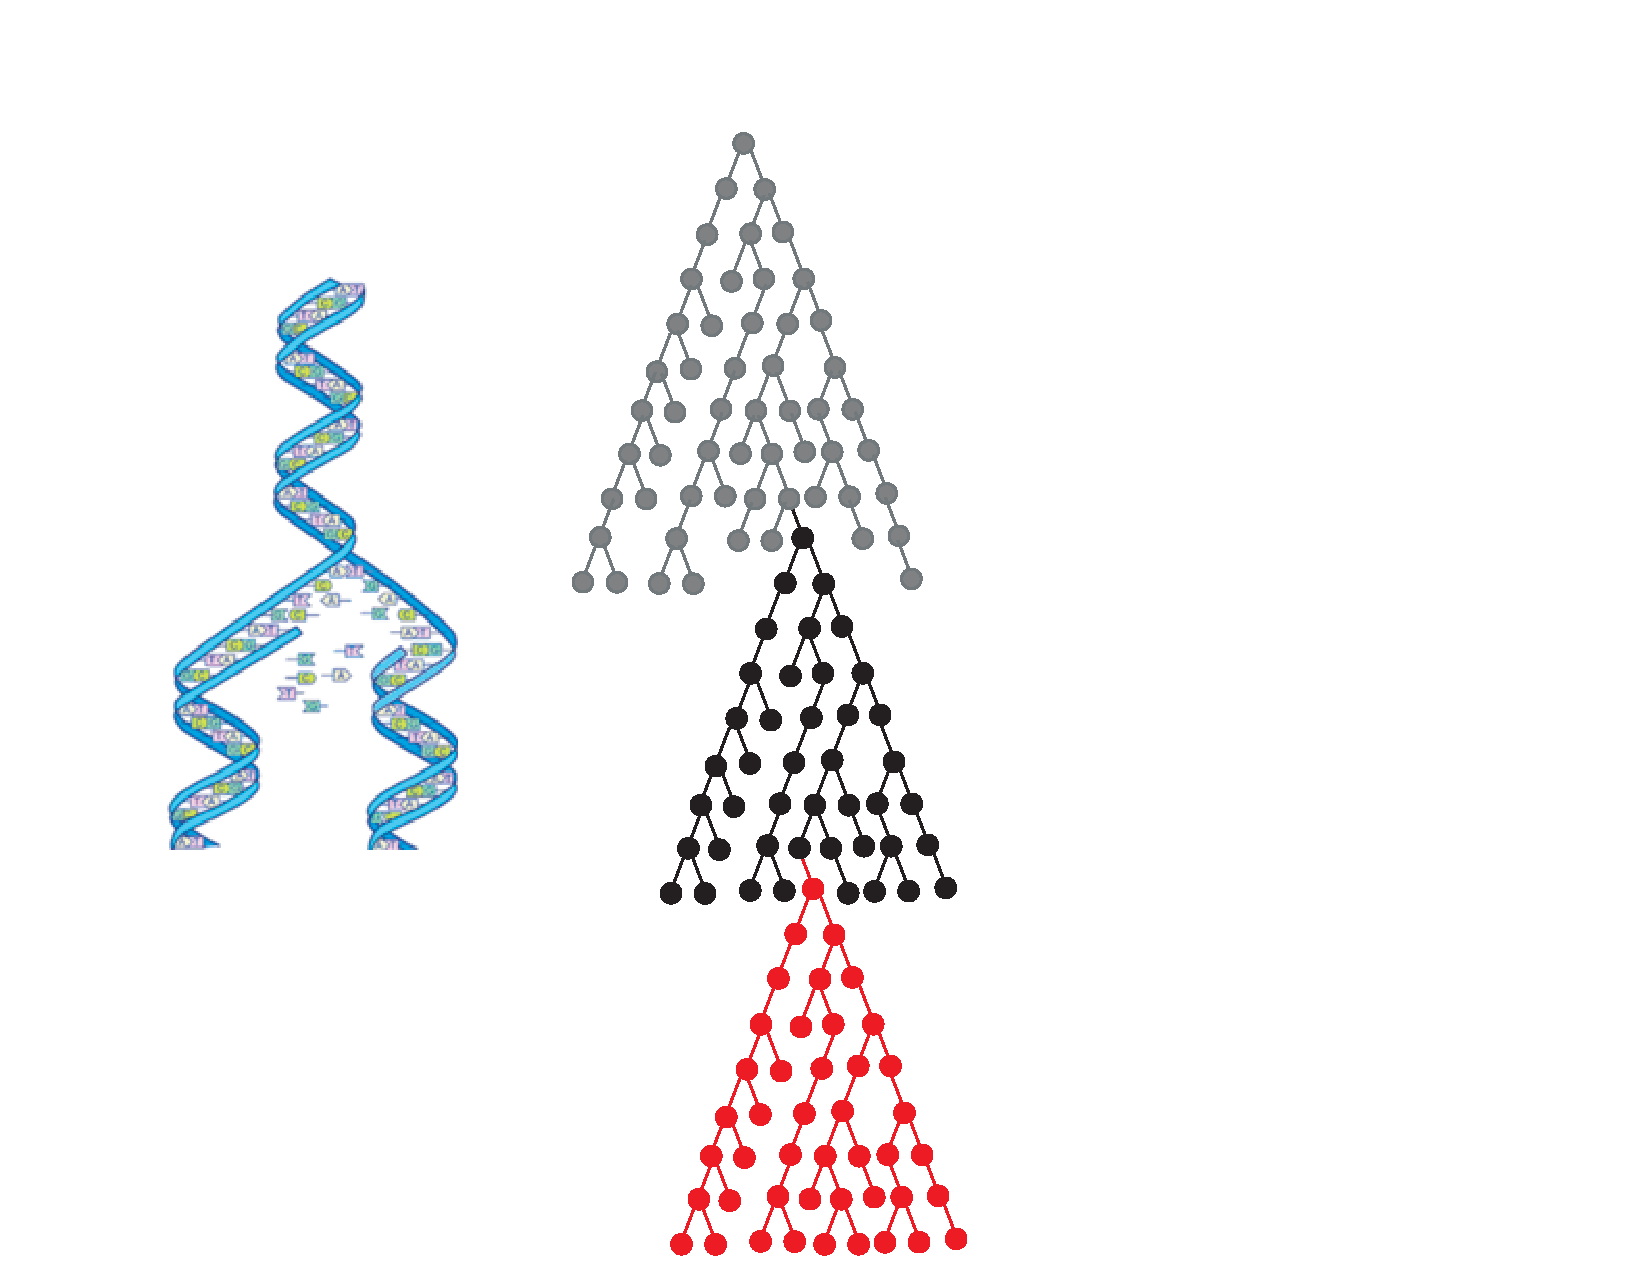
\includegraphics[scale=1.0]{../images/cellPhylogeny.pdf}}}
\end{picture}

\myNewSlide
\section*{Two types of genealogies}
\begin{picture}(0,0)(0,0)  \put(15,-45){\makebox(0,0)[l]{\includegraphics[scale=1.2]{../nonfreeimages/joe/toko_phylo.pdf}}}
\end{picture}

\myNewSlide
\section*{Genealogies within a population}
\unitlength=1mm
\begin{picture}(0,0)(0,0)  \put(15,-55){\makebox(0,0)[l]{\includegraphics[scale=1.2]{../nonfreeimages/joe/wright1.pdf}
}}
\put(65,5){Present}
\put(70,-125){Past}
\end{picture}

\myNewSlide
\section*{Genealogies within a population}
\unitlength=1mm
\begin{picture}(0,0)(0,0)  \put(15,-55){\makebox(0,0)[l]{\includegraphics[scale=1.2]{../nonfreeimages/joe/wright2.pdf}
}}
\put(65,5){Present}
\put(70,-125){Past}
\end{picture}

\myNewSlide
\section*{Genealogies within a population}
\unitlength=1mm
\begin{picture}(0,0)(0,0)  \put(15,-55){\makebox(0,0)[l]{\includegraphics[scale=1.2]{../nonfreeimages/joe/wright3.pdf}
}}
\put(65,5){Present}
\put(70,-125){Past}
\end{picture}

\myNewSlide
\section*{Genealogies within a population}
\unitlength=1mm
\begin{picture}(0,0)(0,0)  \put(15,-55){\makebox(0,0)[l]{\includegraphics[scale=1.2]{../nonfreeimages/joe/wright9.pdf}
}}
\put(65,5){Present}
\put(70,-125){Past}
\end{picture}

\myNewSlide
\section*{Genealogies within a population}
\unitlength=1mm
\begin{picture}(0,0)(0,0)  \put(15,-55){\makebox(0,0)[l]{\includegraphics[scale=1.2]{../nonfreeimages/joe/wright10.pdf}
}}
\put(65,5){Present}
\put(70,-125){Past}
\put(65,15){Present}
\put(70,-115){Past}
\put(-20,-135){Biparental inheritance would make the picture messier, but the genealogy}
\put(-10,-145){of the gene copies would still form a tree (if there is no recombination).}
\end{picture}

\myNewSlide
\section*{terminology: genealogical trees within population or species trees}
It is tempting to refer to the tips of these gene trees as alleles or haplotypes.
\begin{compactitem}
	\item allele -- an alternative form a gene. 
	\item haplotype -- a linked set of alleles
\end{compactitem}
But both of these terms require a differences in sequence.

The gene trees that we draw depict genealogical relationships -- regardless of whether or not nucleotide differences distinguish the ``gene copies'' at the tips of the tree.


\myNewSlide
\unitlength=1mm
\begin{picture}(0,0)(0,0)  \put(-55,-70){\makebox(0,0)[l]{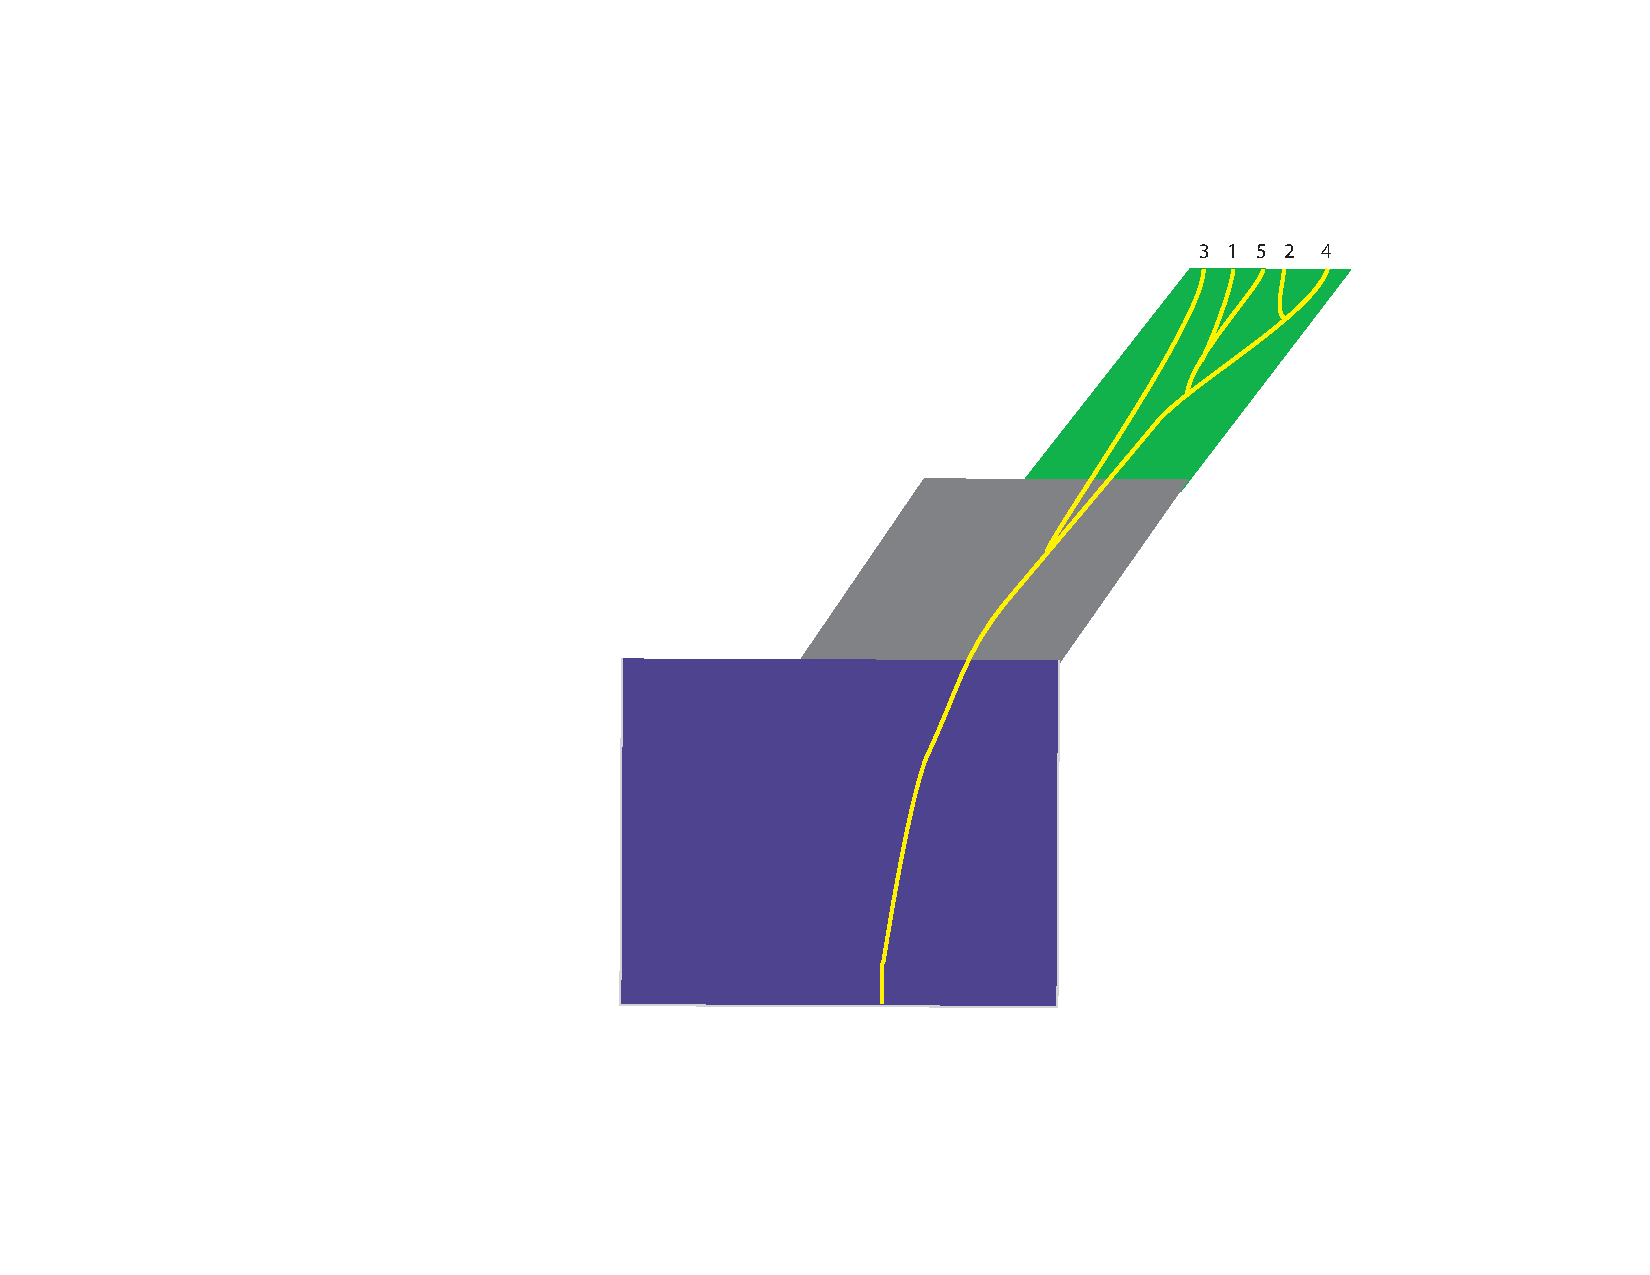
\includegraphics[scale=1.2]{../images/gene_tree_sp_tree_one_sp1.pdf}}}
\end{picture}

\myNewSlide
\unitlength=1mm
\begin{picture}(0,0)(0,0)  \put(-55,-70){\makebox(0,0)[l]{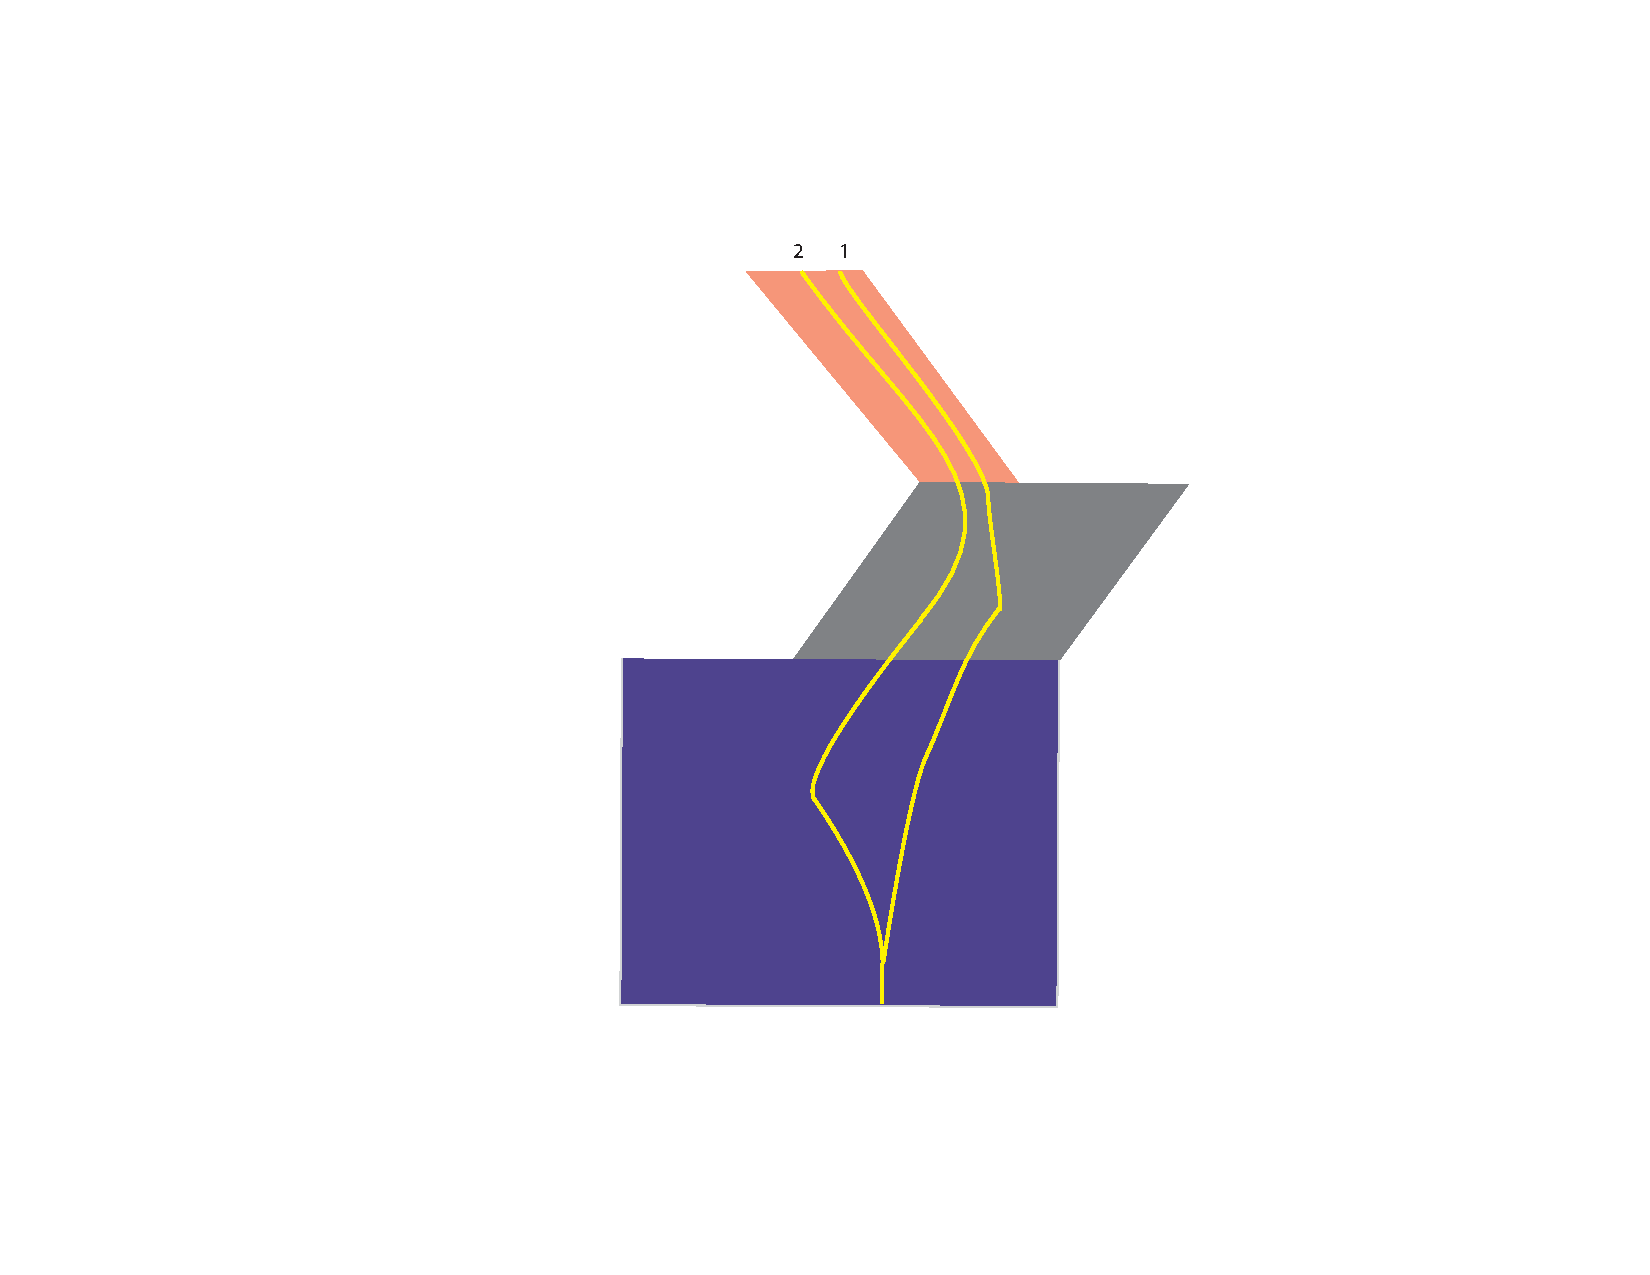
\includegraphics[scale=1.2]{../images/gene_tree_sp_tree_one_sp2.pdf}}}
\end{picture}

\myNewSlide

\section*{A ``gene tree'' within a species tree}
\unitlength=1mm
\begin{picture}(0,0)(0,0)  \put(-55,-70){\makebox(0,0)[l]{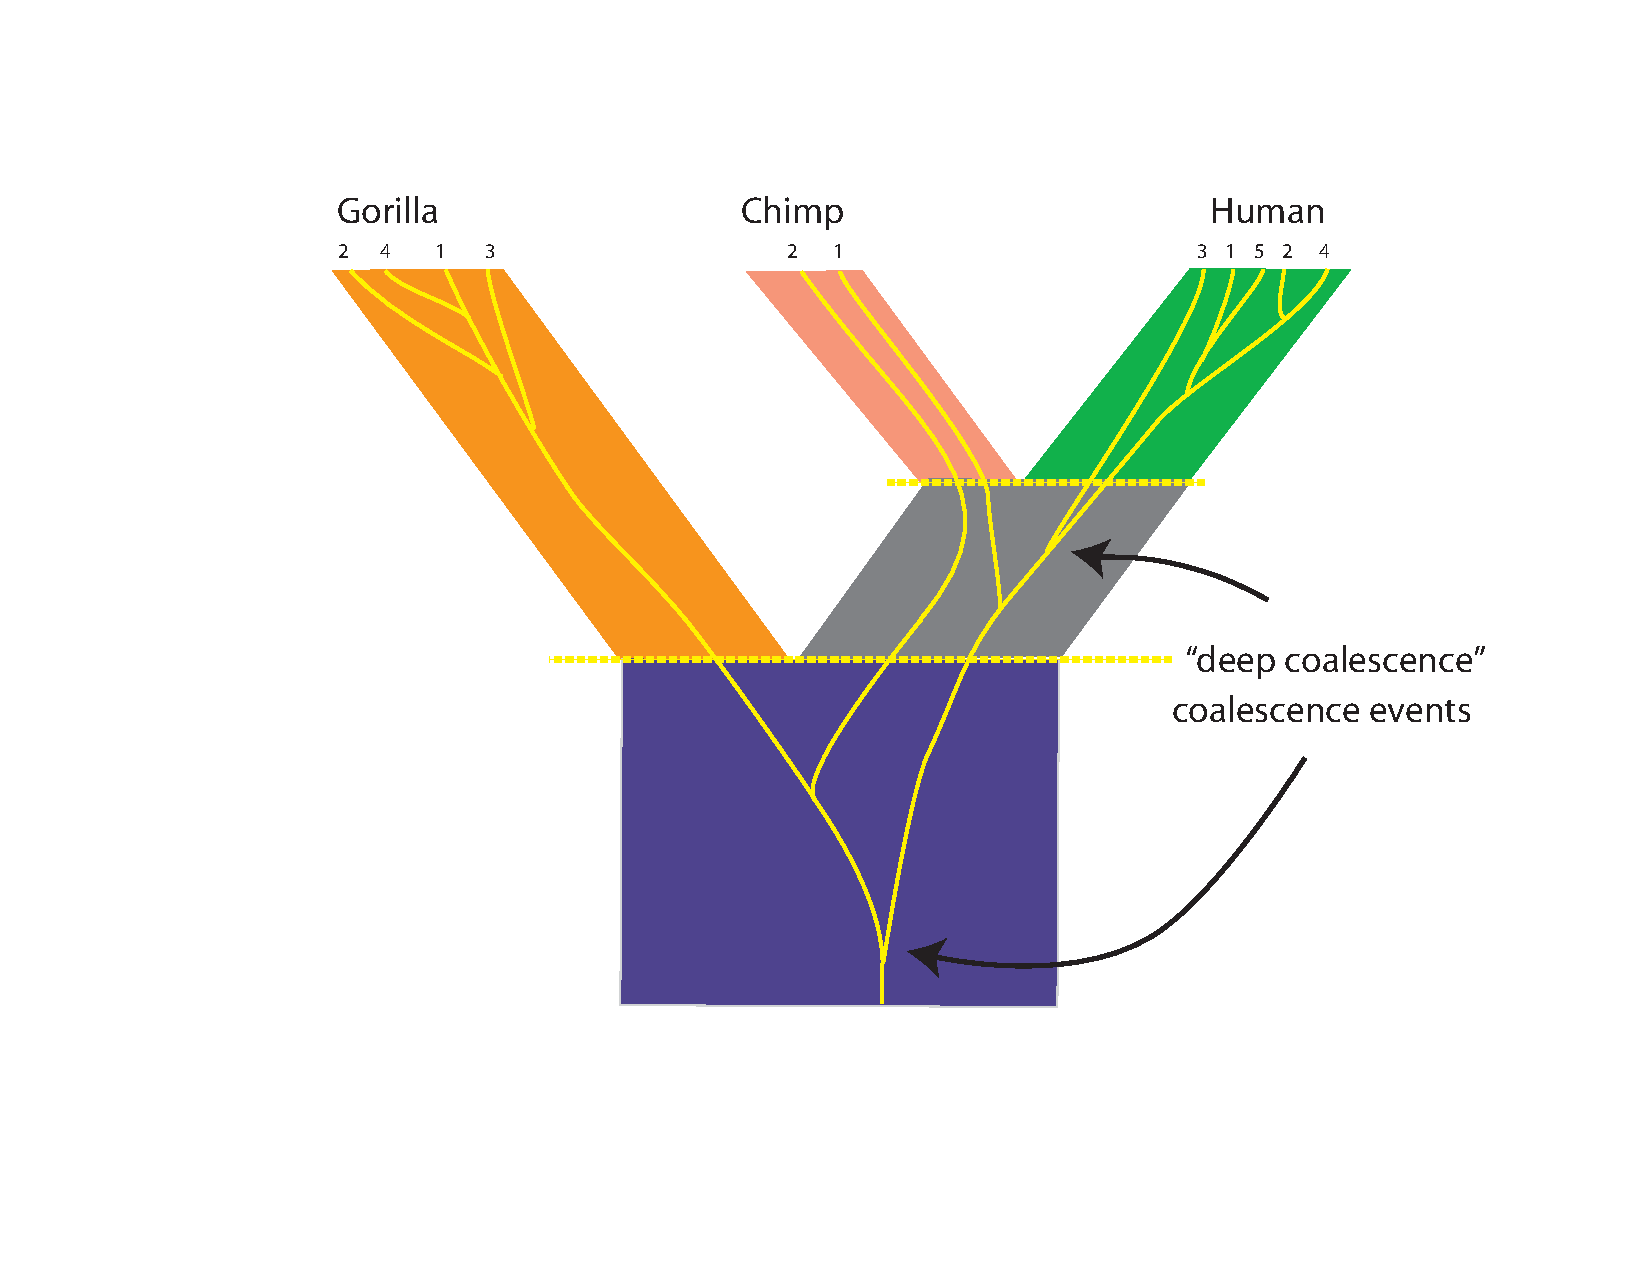
\includegraphics[scale=1.2]{../images/gene_tree_sp_tree.pdf}}}
\end{picture}

\myNewSlide
\section*{terminology: genealogical trees within population or species trees}
\begin{itemize}
	\item coalescence -- merging of the genealogy of multiple gene copies into their common ancestor.  ``Merging'' only makes sense when viewed {\em backwards in time}.
	\item ``deep coalescence'' or ``incomplete lineage sorting'' refer to the {\em failure} of gene copies to coalesce within the duration of the species -- the lineages coalesce in an ancestral species
\end{itemize}


\myNewSlide
\section*{terminology: genealogical trees within population or species trees}
\begin{itemize}
	\item coalescence -- merging of the genealogy of multiple gene copies into their common ancestor.  ``Merging'' only makes sense when viewed {\em backwards in time}.
	\item ``deep coalescence'' or ``incomplete lineage sorting'' refer to the {\em failure} of gene copies to coalesce within the duration of the species -- the lineages coalesce in an ancestral species
\end{itemize}


\myNewSlide
\section*{A ``gene family tree''}
\unitlength=1mm
\begin{picture}(0,0)(0,0)
  \put(-15,-60){\makebox(0,0)[l]{\includegraphics[scale=1.1]{../nonfreeimages/other/OpazoHS2008Fig1.pdf}}}
\put(170,-55){\small Opazo, Hoffmann and Storz}
\put(170,-63){\small``Genomic evidence for}
\put(170,-71){\small independent origins of $\beta$-like}
\put(170,-79){\small globin genes in monotremes }
\put(170,-88){\small and therian mammals''}
\put(170,-97){\small PNAS {\bf 105(5)} 2008}
\end{picture}


\myNewSlide
\unitlength=1mm
\begin{picture}(0,0)(0,0)
  \put(15,-60){\makebox(0,0)[l]{\includegraphics[scale=1.2]{../nonfreeimages/other/OpazoHS2008Fig4.pdf}}}
\put(-15,-150){\small Opazo, Hoffmann and Storz ``Genomic evidence for independent origins of $\beta$-like}
\put(-15,-158){\small globin genes in monotremes and therian mammals'' PNAS {\bf 105(5)} 2008}
\end{picture}

\myNewSlide
\section*{terminology: trees of gene families}
\begin{itemize}
	\item duplication -- the creation of a new copy of a gene within the same genome.
	\item homologous -- descended from a common ancestor.
	\item paralogous --  homologous, but resulting from a gene duplication in the common ancestor. 
	\item orthologous -- homologous, and resulting from a speciation event at the common ancestor.
\end{itemize}


\myNewSlide
Multiple contexts for tree estimation (again):
\begin{table}[htdp]
\begin{center}
\begin{tabular}{|p{5cm}|p{5cm}|p{11cm}|}
& {\bf The cause of splitting} & {\bf Important caveats} \\
\hline
``Gene tree'' & DNA replication & recombination is usually ignored \\
\hline
Species tree Phylogeny & speciation & recombination, hybridization, and deep coalescence cause conflict in the data we use to estimate phylogenies\\
\hline
Gene family tree & speciation or duplication & recombination (eg. domain swapping) is not tree-like \\
\hline
\end{tabular}
\end{center}
\label{default}
\end{table}%



\myNewSlide
\section*{The main subject of this course: estimating a tree from character data}
Tree construction:
\begin{compactitem}
	\item strictly algorithmic approaches - use a ``recipe'' to construct a tree
	\item optimality based approaches - choose a way to ``score'' a trees and then search for the tree that has the best score.
\end{compactitem}
Expressing support for aspects of the tree:
\begin{compactitem}
	\item bootstrapping,
	\item testing competing trees against each other,
	\item posterior probabilities (in Bayesian approaches).
\end{compactitem}
\myNewSlide
\bibliography{../phylo848}

\end{document}
